\chapter{Experimental Setup}
\section{Equipment}
\subsection{ESC Assessment}
The most important component for the analysis in this project is the ESC. Therefore, a thorough assessment of different ESCs and their firmware was made. The criteria to pick the particular board took into account that it is to be used with the Voliro OMAV at the ASL in t ETH Zurich depicted in Figure \ref{fig: mav_photo}. The parameters accounted for as well as the top rated ESCs are shown in Table \ref{tab:tab_escs}. Further analyzed ESCs are show in Appendix \ref{sec:appendix_escs}.

\begin{table}
\small
% \addtolength{\leftskip} {-2cm}
%\addtolength{\rightskip}{-2cm}

\begin{center}
 	\caption{ESC protocols' speeds}\vspace{1ex}
 	\label{tab:tab_escs}
\makebox[\textwidth]{
	 \begin{tabular}{l|rrrrrrrrr}
	 \hline
	ESC Model & Speed feedback & Brake  & Size [mm] & Motors & Protocol & Current Sens & Firmware & Efficiency\\ \hline \hline
	
	Flycolor X-Cross 4in1		&	Telemetry	&	Yes &	42x45x7.5	&	4	&	Dshot	&	Telemetry	&	BlHeli\_32	& 	Sine Mod\\
	Lumenier Elite 4in1			&	Telemetry	&	Yes &	43x46x7.5	&	4	&	Dshot	&	Telemetry	&	BlHeli\_32	&	Sine Mod\\
	Holybro Tekko32 F3 Metal	&	Telemetry	&	Yes	&	42x42x4		&	4	&	Dshot	&	Analog		&	BlHeli\_32	&	Sine Mod\\
	Myxa by Zubax				&	UAVCAN		&	Yes	&	57x38x24	&	1	&	UAVCAN	&	UAVCAN		&	Sapog v2	&	FOC\\
	Holybro Koleta20			&	UAVCAN		&	Yes	&	40x27x5		&	1	&	UAVCAN	&	UAVCAN		&	Sapog v2	&	FOC\\
	\end{tabular}
}

\end{center}
\footnotesize{NOTE: All ESCs that support Dshot in this table support all analog protocols and Bidirectional Dshot}
\end{table}

Therefore, we can see that there are two trends of high-performance ESCs. The first one relates to the most modern ESCs used in drone racing. They are very similar since they are mostly manufactured to use the BlHeli\_32 firmware. This firmware, allows for multiple parameter modification via the software BlHeliSuite (see Appendix \ref{sec:firm_blheli} for instructions). Given their modularity, they can be made into very small boards. For instance, they now come in 4 in 1 boards (i.e. one board includes 4 ESCs). The other group of high-performing ESCs use UAVCAN as communication protocol with the FC. This gives the advantage of less cabling. They use FOC which makes them more efficient than Sine Modulation versions specially at low rotor speed (below 1000 RPM). These also have possibility of on-board speed control, but it does not include any feed-forward prior.  The Holybro Tekko32 F3 ESC was then selected for investigation due to the wide variety of protocols it supports, it's multiple rotor support, good heat-sinking and flexibility to change parameters. Please refer to Section \ref{sec: esc_dig_prot} for a more thorough description of Dshot, Bidirectional Dshot and UAVCAN protocols.

\subsection{Overall setup}

The rig shown in Figure \ref{fig:exp_setup} was setup for testing purposes and included the following core components:
\begin{itemize}
	\item 2 BLDC motors by KDE Direct model 2315XF-885Kv 14 poles.
	\item 1 clockwise Hobbyking Propeller 9in diameter 4.7in pitch.
	\item 1 counter-clockwise Hobbyking Propeller 9in diameter 4.7in pitch.
	\item 1 Tekko32 F3 Metal ESC.
	\item 1 6S LiPo battery.
	\item Pixhawk 4 flight controller
	\item Laptop (running Ubuntu 18.04 for firmware compilation).
	\item Support towers to attach motors.
\end{itemize}
\begin{figure}
    \centering
    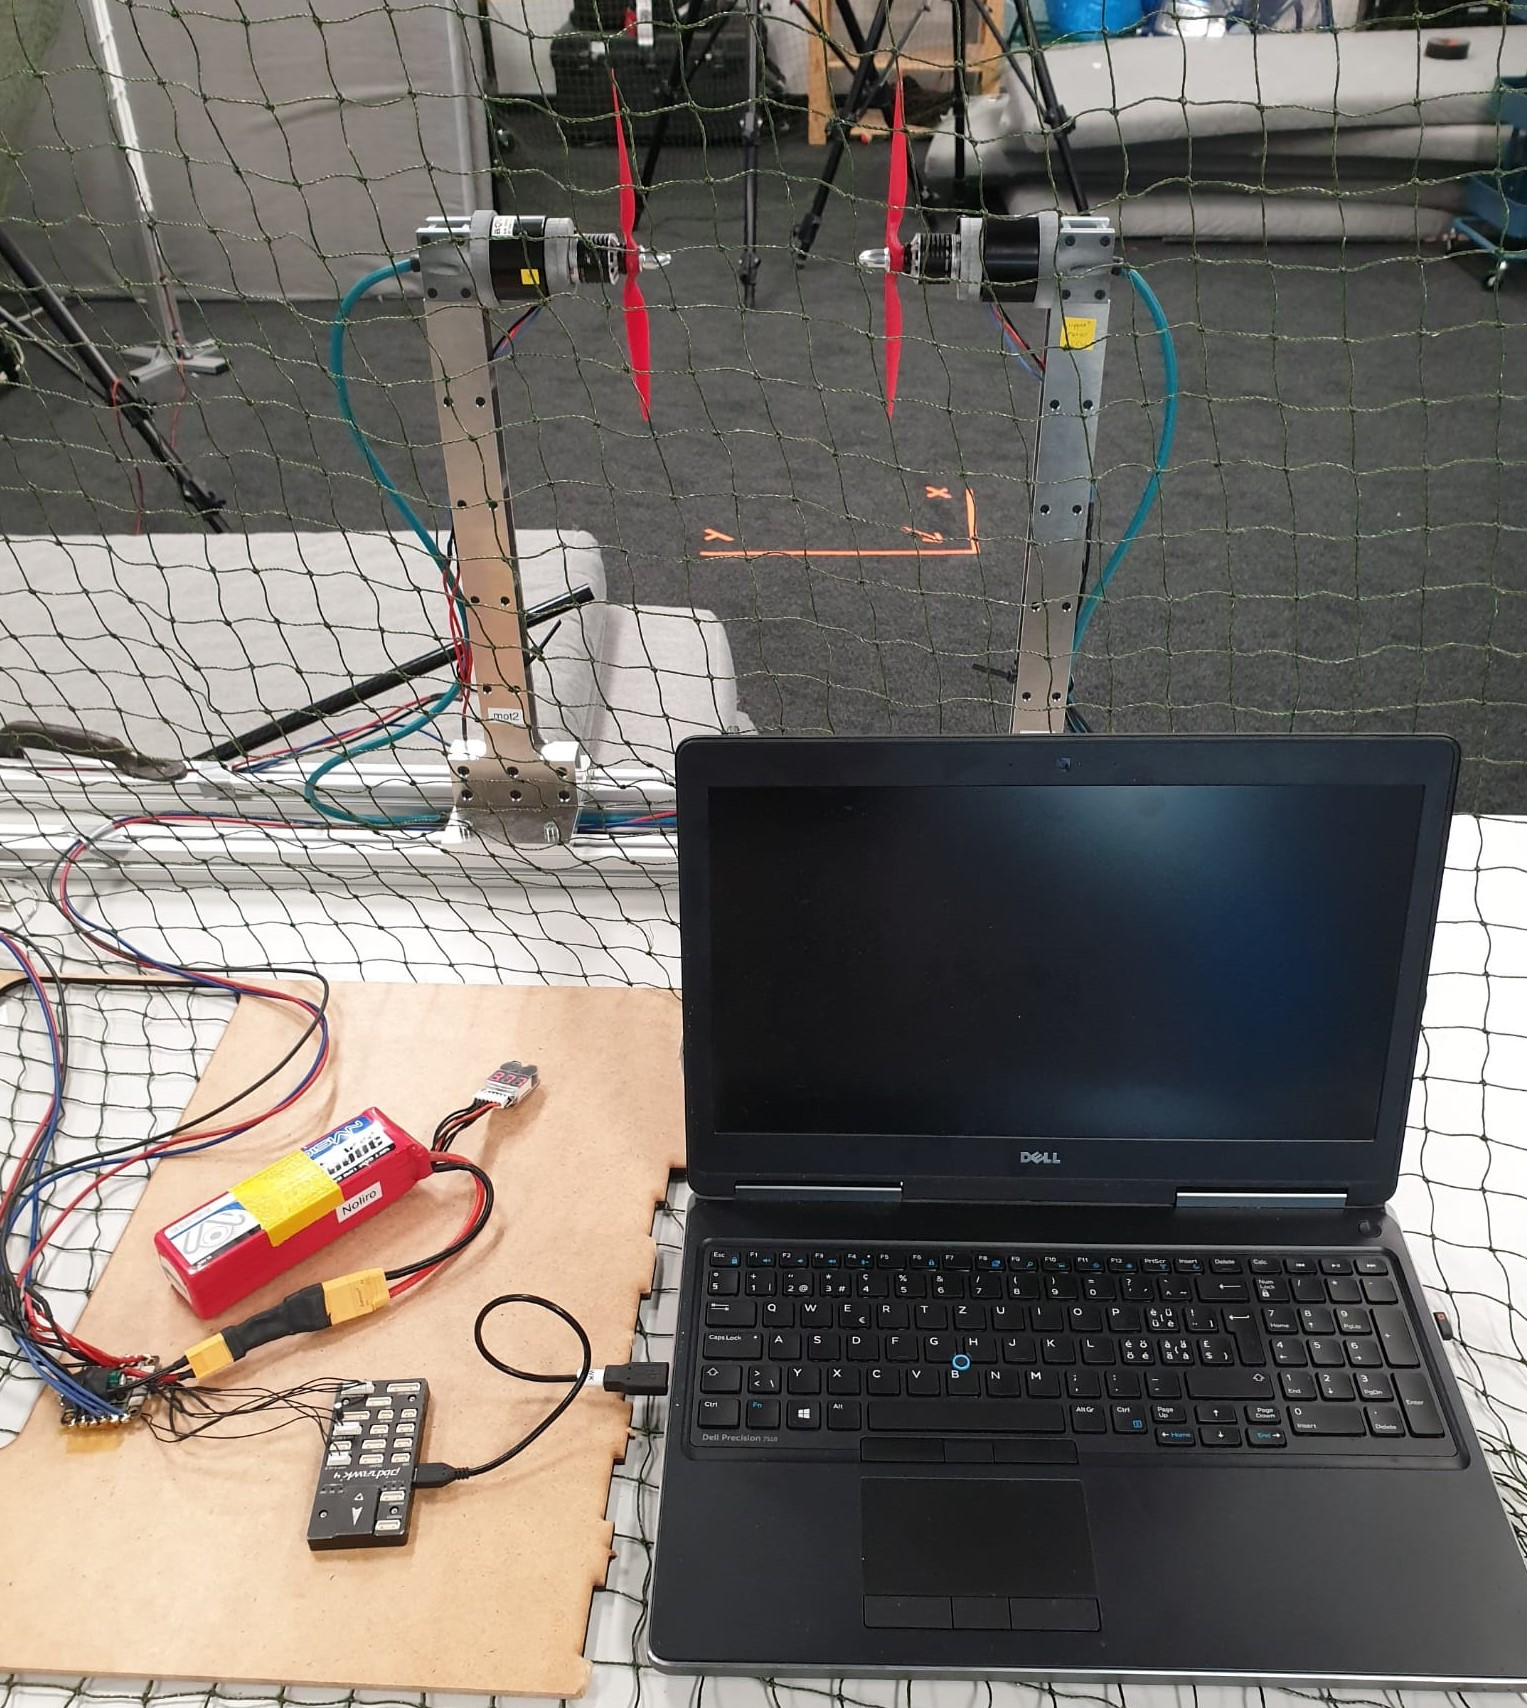
\includegraphics[width=0.9\textwidth]{images/setup_photo.png}
    \caption{Experimental setup}
    \label{fig:exp_setup}
\end{figure}

\section{Software toolboxes}


\section{Software developed}